\chapter{Experimental Design and Setup}

\label{chapter-approach-to-study}

\section{Approach to the Study}

Several neural network models are used in the project. One is the GRU sequence-to-sequence model, another the Transformer model for a generative chatbot and finally, the Generative Pre-Training 2 model.

A rewrite for the Transformer or GPT2 model is not attempted.

In this project the chatbot code is loaded onto small single board computers as much as possible. The Raspberry Pi and the Jetson Nano are considered to be small single board computers.

Models are trained using the Pytorch and Tensorflow libraries. These models are responsible for taking in English sentences and producing English output. Another part of the typical Raspberry Pi setup includes another neural network component. Speech to text models, which this application requires, rely on large neural network resources. Speech to text resources, supplied by Google on the Google Cloud are used. To include speech to text libraries locally on the Raspberry Pi would be too costly in computation time and resources like RAM. It would also be complicated to implement technically. It could easily comprise an entire project on its own.

%The speech to text resources supplied by Google cost money. To use the service you need to have a billing account with Google.

The speech to text service used here and the Raspberry Pi memory limitations are problematic. The chatbot function could be served from some faster machine located somewhere on the Internet. It would entail two calls from the Raspberry Pi for every sentence.% complicates things. % and also has a time overhead. 

%There are several models to test. 
%To test them all would require several servers. In addition they 
Another problem is the models use both Pytorch and Tensorflow. Tensorflow has `tensorflow-model-server' for serving models, but Pytorch has no equivalent. %Testing them all requires several servers.

It is important to note that the large GPT2 model specifically could be served from a remote computer and would operate faster. Currently on the Raspberry Pi, decoding a single sentence with the 117M parameter GPT2 takes approximately 13 seconds. However, it is preferred to install these trained models on the Raspberry Pi directly.

The 117M parameter GPT2 model fits on a Jetson Nano and can produce the response to a question in two or three seconds. The Nano is not much bigger than a Raspberry Pi.

If every Raspberry Pi computer in this project was replaced with Jetson Nano computers, all of them would respond quickly and with only a natural pause before each reply.

\section{Hardware Installation Overview}



\begin{table}[H]
	
	\begin{center}
		
		
		\begin{tabular}{llllll}
			
			Model Name    & File  & RAM  & RAM    & Hand & Board \\
			&  Size & Train   & Inference    & Trained &   Type \\
			\hline
			\hline
			Seq-2-Seq/Tutorial & 230 M     & 1.1 G & 324 M             & YES  &  Pi 3B \\
			Transformer/Persona   & 25 M      & 556 M & 360 M          & YES  & NONE \\
			Transformer/Movie \dag \dag  & 550 M      & 6.5 G & 500 M  & YES    & Pi 4B  \\
			GPT2 small - 117M \dag   & 523 M  & -   & 2.0 G         & NO     &  Pi 4B/Nano \\
			\hline
		\end{tabular}
		
		\bigskip
	\end{center}
		\dag \ a large GPT2 model exists, but it is not small enough to fit on a Raspberry Pi or Jetson Nano.
		
		\dag \dag \ This is referred to as the `larger' Transformer model, though it is smaller than the smallest GPT2 model.
		
	%\end{center}
	
	\label{fig:modeloverview}
	\addcontentsline{lot}{section}{Hardware Overview}
\end{table}


A short description for each row is provided below.

\begin{itemize}
	\item \textbf{Sequence-to-Sequence - Tutorial} This model uses the sequence-to-sequence architecture and the Gated Recurrent Unit component. Here the slightly modified version of the sequence-to-sequence model is based on the tutorial from Inkawhich et al \cite{2018Inkawhich}, using the Movie Dialog corpus with a hidden size of 500 units. This model was used in one Raspberry Pi installation.
	
	\item \textbf{Transformer - Persona} This model uses a Tensorflow Transformer architecture. Coding is used to interface with the text-to-speech and speech-to-text libraries. Additional coding loads project corpus data during this training. The model parameters describe a rather small model and uses the Persona Dialog corpus. It uses 2 layers, 4  heads, and a hidden size of 128. This model was not permanently installed. It is not on a Raspberry Pi board.
	
	\item \textbf{Transformer - Movie} This model is based on the Transformer model above but uses the Movie Dialog corpus and a larger parameter set. In many ways this model is bigger than the one that uses the Transformer and the Persona corpus. It uses 6 layers, 8 heads, and a hidden size of 512. This was used in one Raspberry Pi installation.
	
	\item \textbf{GPT2 small} This model was downloaded from the internet, and fits on a Raspberry Pi 4B with the 4GB RAM option. It also fits on a Jetson Nano. Some modification was made so that model output was suitable. It uses 117M parameters, with 12 layers and a hidden size of 768. This model was used in one Raspberry Pi installation and one Jetson Nano installation.
\end{itemize}

\section{Setup}

Linux computers are used, sometimes with \ac{GPU} hardware for parallel processing. The Python programming language is used. Code from this project can be run with the 3.6 or 3.7 version of Python.

When the project was started, some programming with Keras was done using Tensorflow as a backend. Keras was later discarded in favor of Pytorch and Tensorflow, although Tensorflow and Pytorch do not work together. Pytorch as a library is still under development at the time of this writing.

Some of the Generative Pre-Training 2 code uses Pytorch, and some uses Tensorflow. A repository on Github uses the GPT2 trained model with Pytorch instead of Tensorflow.

Github is used as a code repository. Code corresponding with this paper can be found at: \href{https://github.com/radiodee1/awesome-chatbot}{https://github.com/radiodee1/awesome-chatbot} . 

As an experiment, a rewrite for the sequence-to-sequence GRU was coded with little success. There is no rewrite for the GPT2 code from the Tensorflow or Pytorch repository.

\subsection{Graphical Processing Unit vs. Central Processing Unit}

A CPU has a number of cores, usually between 2 and 16. A CPU is designed to execute one command at a time, and has limitations when it comes to executing matrix multiplication. %Matrix multiplication using a CPU can take a long time.

GPUs, Graphical Processing Units, have the ability to address tasks like matrix multiplication with many more processing units at once. They speed up parallel processing and are a benefit to neural networking training.% tasks that the CPU doesn't have.

Unfortunately, state of the art neural network models are larger than the capacity of a single GPU. Some models are trained on many GPUs simultaneously. It is not uncommon for a model to train on a computer with eight GPU cards for many days. It is possible to rent time on Amazon Web Services or Google cloud to do this training, but it can be costly.

This is addressed partially by the Transfer Learning scheme, where an already trained version is accessible to the public. The programmer downloads the model and fine tunes it to suit the task.

Here, the GRU based sequence-to-sequence model and the Tensorflow based Transformer model were trained from scratch on a CPU laptop. In the case of the Transformer, several days were required for training. In the GRU example the model trained in less than an hour.

\subsection{Raspberry Pi}

A Raspberry Pi is a small single board computer with an `arm' processor. There are several versions on the market, the most recent of which has built-in wifi and on-board graphics and sound. The memory for a Raspberry Pi 3B computer is 1Gig of RAM. Recently available, the Raspberry Pi 4B computer has 4Gig of RAM.

It is the intention of this project to install several chatbot models on Raspberry Pi computers. All chosen models must be small enough in file size to fit on the Pi.

%Several resources must be made available. 
Pytorch needs to be compiled for the Pi. Speech Recognition and Text To Speech must be available. Early tests using Google\textquoteright s \ac{SR} and TTS services show that the Pi can support them. 


%Google's SR service is expensive. 
Details for setting up Google's SR and TTS functions are found in the README file of this project\textquoteright s Github repository.

The chosen model is trained on the desktop computer and then the saved weights and biases are transferred to the Raspberry Pi platform. The Pi is not required to do any training, only inference. 

\begin{figure}[H]
	\begin{center}
		\includegraphics[scale=0.1]{diagram-pic01}
		
		
	\end{center}
	\caption[Raspberry Pi]{Raspberry Pi 4B - Modified with push button and indicator lights.}
	
	
\end{figure}

\subsection{Jetson Nano}

The Jetson Nano is another small single board computer. Though it has no WiFi, it is outfitted with an NVIDIA Graphical Processing Unit. 

While the development computer uses x86\_64 and the Raspberry Pi uses ARMv7, the Nano uses aarch64. It is based on the ARM architecture with 64 bit memory units. ARMv7 uses 32 bit memory units.

It is not much bigger than a Raspberry Pi, has four Gigabytes of memory, and an Ubuntu based operating system. The operating system has Python 3.6 and special NVIDIA GPU libraries pre-installed. Pytorch can be installed.

In normal mode the board has an HDMI connector providing both video and audio output. For the project, the board was outfitted in headless mode, % In headless mode the 
requiring USB connectors to provide audio input and output.

Because it does not have on-board WiFi, a WiFi board must be installed, or a WiFi USB dongle used.

Google's Speech Recognition and Text-To-Speech software works on this platform. The Nano did not need to be employed for any training. It was used solely for inference.

\begin{figure}[H]
	\begin{center}
		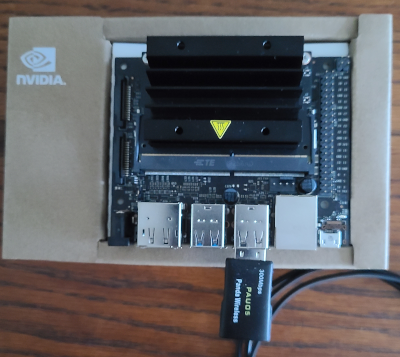
\includegraphics[scale=0.9]{diagram-jetson-nano-02}
		
		
	\end{center}
	\caption[Jetson Nano]{Jetson Nano without case.}
	
	
\end{figure}

\subsection{Reply Time}

The Google Text-To-Speech software takes negligible time to execute.

The Speech Recognition software takes one or two seconds to execute, as each audio sample must be sent to a Google server for translation into text. Because performance relies on network speeds, execution time is uncertain.

The actual model is responsible for taking question text, and returning an appropriate answer in text form to the calling function. Each model is, in turn, connected to the same SR and gTTS software.

On the development computer most of the models tested take little or no time to execute. On the Raspberry Pi only the GRU model executes instantaneously. Each of the other models requires more.  %s some time to reply to a basic request.

On the Jetson Nano, the largest installed model, the 117M GPT2 model requires a few seconds to execute. %The other models require less. %are smaller than the GPT2 model, and so all would take less than two seconds.

Reply time is determined by inference time and time for general SR server calls.

All models' first reply is longer. This is normal and is explained by the program's need to load a large set of matrices for the first reply. This loading overhead is not needed in the subsequent program replies. % The matrices only need to load once.

\label{setup-reply-time}

\begin{table}[H]
	
	\begin{center}
		
		
		\begin{tabular}{lllll}
			
			Model Name    & Board  & SR  & Reply    & Total  \\
			&  Type & Time  & Time    & Time  \\
			\hline
			\hline
			Seq-2-Seq/GRU Tutorial & Pi 3B     & 2s & 0s             & 2s   \\
			Transformer/Movie Corpus & Pi 4B      & 2s & 5s  & 7s      \\
			GPT2 small - 117M   & Pi 4B     & 2s   & 13s         & 15s      \\
			GPT2 small - 117M   & Jetson Nano & 2s   & 3s         & 5s      \\
			\hline
		\end{tabular}
		
		\bigskip
	\end{center}
	
	
	\label{fig:time-compare}
	\addcontentsline{lot}{section}{Time Comparison}
\end{table}


\subsection{Tensorflow vs. Pytorch}

Tensorflow is a Google library. Pytorch has it's roots with Facebook. Both run in a Python environment. While Pytorch offers Python objects that can be combined to create a neural network, Tensorflow has different pieces, but they cannot be examined as easily at run time.

Tensorflow has a placeholder concept for inputting data and their results. Placeholders are set up at design time and are used to access data at run time.

Pytorch objects interact with Python more easily, allowing print statements in the code to show data transferred from one object to another. This is possible at run time.

Tensorflow has a tool, called Tensorboard, good for visualization which can print out graphs of data while the model trains. 

\subsection{Speech and Speech To Text}
\label{speech-and-speech-to-text}

Google has Python packages that translate text to speech and speech to text. In the case of text to speech the library is called `\ac{gTTS}.' In the case of speech to text the library is called `google-cloud-speech'. 

The gTTS package is simple to use and can be run locally without connection to the Internet. The google-cloud-speech package uses a google cloud server to take input from the microphone and return text. For this reason it requires an Internet connection and an account with Google that enables Google Cloud API use. %Google charges the user a small amount for every word that they translate into text. 

Both of these resources work well on the Raspberry Pi, but configuring STT for the Pi is not trivial. The user must register a billing account with Google cloud services. In return for this registration, the user is able to download a JSON authentication file that must be copied to the Raspberry Pi. 

Furthermore, an environment variable, called `GOOGLE\_APPLICATION\_CREDENTIALS' must be set that points to the authentication file. It must be set along with the launching of the neural network model.

The operating system on the Raspberry Pi is based on Debian Linux. In this system a file is run immediately after the basic system starts up, called `\textbf{/etc/rc.local}'. It is sufficient to put the environment variable there and follow it with the launching of the model. The setting of the environment variable is combined with the launching of the program in a single line of code.


\subsection{Corpus Considerations}

Several data sets have been collected for the training of a chatbot model. First is a corpus of movie subtitles, then the corpus described by Mazar{\'{e}} et al \cite{DBLP:journals/corr/abs-1809-01984}. This corpus is specifically designed to train the chatbot task. This is referred to as the Persona corpus.

For the Persona corpus, the text is organized into `JSON' objects with several different repeated labels. Some of the text is meant to be used in question and answer pairs. Sentences labeled as `history' are most suited to this task. %These values are recorded only and discard other labels.

The WebText corpus, culled from Reddit, is used for the training the GPT2 model. This material is not used in this paper directly, but it is a part of the success of the GPT2. This corpus is 40Gig of data.

\subsection{Chatbot vs. Smart Speaker}

A chatbot is a computer program that takes input from the user and replies as if it were a human. A chatbot is most often encountered on web sites and html pages. Input is usually in the form of typed text. Output is usually in the form of text on the screen.

A smart speaker is a term referring to a physical object that has a speaker and a microphone and some kind of computer that takes spoken input. Often the smart speaker controls lights or other appliances in a home. It will, on occasion, reply with a human voice. 

For this paper the term smart speaker is used for a small computer that speaks and can be spoken to. The smart speakers in this paper do not control household appliances.

\section{ARMv7 Build/Compile}

\subsection{Pytorch `torch' Library 1.1.0 For ARMv7}
The Pytorch library is compiled for the Raspberry Pi. Several virtualization techniques are used to do this compilation. The result of those efforts is a Pytorch Python 3.7 library. % for the Raspberry Pi.

On their web site Milosevic et al \cite{2018Milosevic} compile Pytorch 1.1.0 for the Raspberry Pi. The instructions called for constructing a change-root environment where a Fedora Core 30 linux system was set up. Then the ARMv7 system was used to compile the Pytorch library. % for the 1.1.0 version.

The production laptop used for development ran Ubuntu Linux. For this reason a Virtualbox emulation was set up with Fedora Core 30, and the change-root environment.% The library was compiled there successfully. 

There are two problems with the resulting Python package. First there is a Python error when importing the torch library, that reads `ImportError: No module named \_C.' 

The build process for ARMv7 creates misnamed shared object files. To correct this, the misnamed files must be found, copied, and suitably renamed. The same outcome could be assured by making symbolic links to the misnamed files with proper names.

Three misnamed files can be found at `\textbf{/usr/lib/python3.7/site-packages/torch/}.' Named with the same convention, all have the ending `.cpython-37m-arm7hf-linux-gnu.so.' They must be renamed with the shorter `.so.' The files should be named `\textbf{\_C.so},' `\textbf{\_dl.so},' and `\textbf{\_thnn.so}.'

%This takes care of the `ImportError'. 
The second problem occurs because, the GLIBC in the change-root environment does not match the GLIBC library in the Raspberry Pi Raspbian distribution. This produces the following error: `\textbf{ImportError: /usr/lib/x86\_64-linux-gnu/libstdc++.so.6: version `GLIBCXX\_3.4.26' not found}.' This is solved by rebuilding the package with Fedora Core 29 instead of 30. 
 
\subsection{Pytorch `torch' Library 1.4.0 For ARMv7}
The Pytorch library is recompiled for the Raspberry Pi using Debian virtualization techniques. Because Ubuntu is a Debian derivative it is not necessary to run the process in a Virtualbox container. 

In addition, the files are properly named and there is no need to change anything in the directory `\textbf{/usr/lib/python3.7/site-packages/torch/}'. 

Compiling took five hours. Time spent with the Virtualbox container was more than twice that. The time spent on the Raspberry Pi executing a single Generative Pre-Training 2 question and answer remained 13 seconds. There was no gain in that respect.

There were several small hurdles to completing the compilation. First, the `debootstrap' command needed to be employed. Because Debian Stretch was used as the host operating system, the GLIBC compatibility problem was not faced. 

Second, some dependencies needed to be installed on the `chroot' environment for Pytorch to compile. One was `libblas3.'

Third, Python 3.7 needed to be built on Stretch because program repositories used Python 2.7 and 3.5. Furthermore, the Raspbian operating system on the Raspberry Pi 4B is based on Debian Buster and used Python 3.7. After that the Git program needed to be compiled. Although Git on Stretch had an issue that was fixed upstream, it was important to use Stretch because of the GLIBC issue. Instead of using the upstream fix, Git was compiled from source. 

Finally, for Pytorch, CUDA and distributed computing was disabled as neither exists on the Raspberry Pi.

\subsection{Docker Container `tensorflow-model-server' For ARMv7}
The Google machine learning library for Python uses a standalone program called `tensorflow-model-server' for serving all Tensorflow models in a standard way. The program has not officially been compiled for ARMv7. A Docker image does exist that will run on ARMv7 (Maciejewski et al \cite{2020Maciejewski}).

Docker was run on the Raspberry Pi in the ARM environment. This terminal excerpt shows this. These commands were executed on the Pi.

\begin{verbatim}
$ sudo apt-get update
$ sudo apt-get upgrade
$ curl -fsSL test.docker.com -o get-docker.sh 
$ sh get-docker.sh
$ sudo usermod -aG docker $USER
\end{verbatim}

To take advantage of Docker one needs to log out and then log in again.

A version of the Docker Container for the model server was run on the Raspberry Pi. A script was written that interacted with the existing ARMv7 container. % The author of the original container is Erik Maciejewski \cite{2020Maciejewski}.

`Tensorflow-model-server' was used on the localhost Internet address, 127.0.0.1, with a port of 8500. While tensorflow-model-server is meant for serving neural network resources on the Internet, it was used on the Raspberry Pi.

